\subsubsection{Example Unification}

Suppose we want to join two states of a FunArray \texttt{\string{0 i\string} $\top$ \string{n\string}} and \texttt{\string{0 i-1\string} [0,0] \string{1 i\string} $\top$ \string{n\string}?}, as in \cite[example 8]{cousot2011}.


\begin{center}
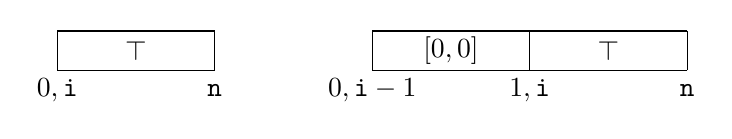
\begin{tikzpicture}
    \draw (0,0) -- (2,0);
    \draw (0,0.5) -- (2,0.5);

    \draw (0,0) -- (0,0.5);
    \draw (0,-0.25) node {$0, \mathtt{i}$};

    \draw (1,0) node[anchor=south] {$\top$};

    \draw (2,0) -- (2,0.5);
    \draw (2,-0.25) node {$\mathtt{n}$};


	\draw (4,0) -- (8,0);
    \draw (4,0.5) -- (8,0.5);

    \draw (4,0) -- (4,0.5);
    \draw (4,-0.25) node {$0, \mathtt{i}-1$};

    \draw (5,-0.05) node[anchor=south] {$[0,0]$};

    \draw (6,0) -- (6,0.5);
    \draw (6,-0.25) node {$1, \mathtt{i}$};

	\draw (7,0) node[anchor=south] {$\top$};

	\draw (8,0) -- (8,0.5);
    \draw (8,-0.25) node {$\mathtt{n}$};    
\end{tikzpicture}
\end{center}